\documentclass[conference]{IEEEtran}
\usepackage{amsmath,graphicx,booktabs,microtype,url}
\graphicspath{{../../figures/paper1/}}

\begin{document}

\title{The Representation Utility Gap in Audio LLMs for Clinical Speech}

\author{\IEEEauthorblockN{Chaitanya Parwatkar, Minoo Ahmadi, Nima Kelidari, Ashutosh Chaubey, Mohammad Soleymani}
\IEEEauthorblockA{University of Southern California, Los Angeles, CA, USA}}

\maketitle

\begin{abstract}
Audio language models answer clinical questions about a recording directly: is this speaker
depressed, cognitively impaired, or has Parkinson's? We test whether those answers use what the
models hold. On three conditions where the words carry almost nothing, some, or most of the diagnosis,
linear probes read the disease from the frozen encoder of an audio LLM at 0.78 to 0.96 AUC, while the
same model's answers on the same clips sit at 0.54 to 0.66. The answer follows the words:
transcript-only input scores the same or better, synthetic speech carrying the same words scores the
same as the patient's voice, and when the words contradict the diagnosis six of nine models fall below
chance. Seven fixes that leave the weights untouched do not close the gap; training the smallest parts
does, a linear readout reaching 0.78 and a retrained projector 0.80 where the answer reads 0.62. The
gap replicates on a second Alzheimer's dataset and on the ADReSS-2020 split. The diagnosis is present
in the model's states; the step that maps them to an answer does not use it.
\end{abstract}

\begin{IEEEkeywords}
audio language models, clinical speech, probing, Alzheimer's disease, Parkinson's disease, depression
\end{IEEEkeywords}

\section{Introduction}\label{sec:intro}

Speech carries measurable signs of Parkinson's disease, depression and Alzheimer's disease, and
audio language models (audio LLMs) now answer clinical questions about a recording in natural
language. That makes them attractive for screening: one model, one prompt, no task-specific
training. Probing studies add to the appeal by showing that speaker state is richly encoded across
the layers of these models \cite{probing}.

\begin{figure}[!t]
\centering
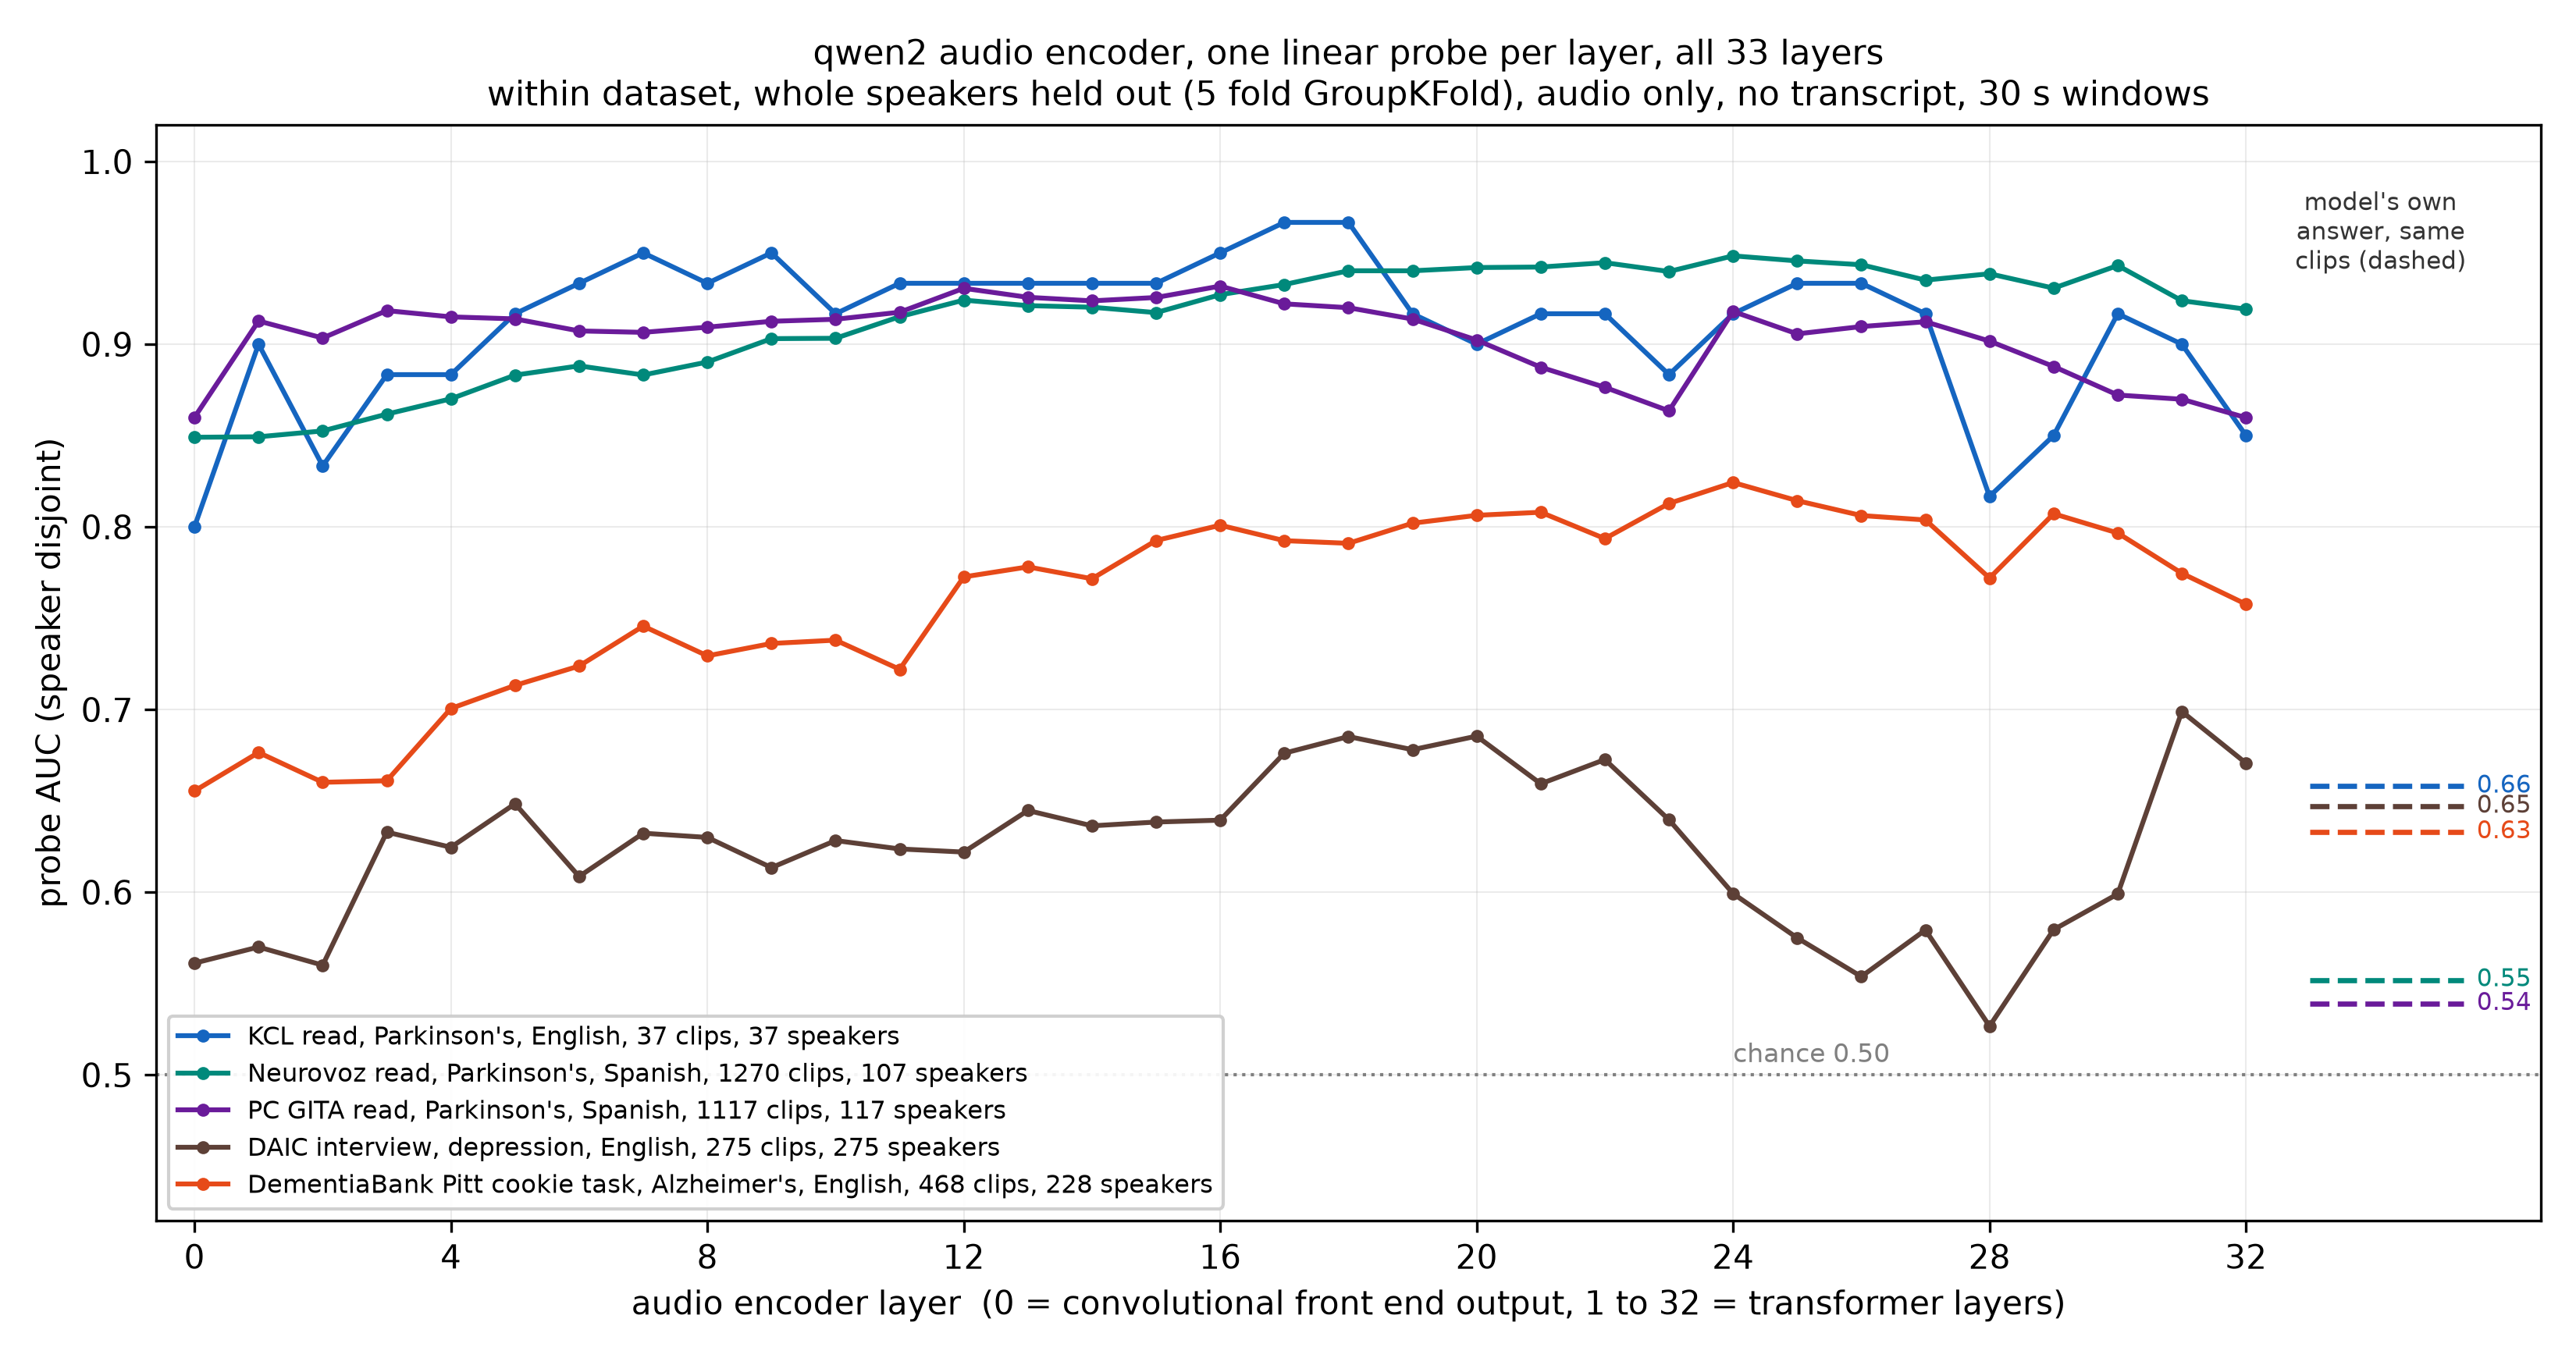
\includegraphics[width=0.8\columnwidth]{plot1_encoder_layers.png}
\caption{A linear probe on every encoder layer of qwen2-audio (solid) against the model's own
answer on the same clips (dashed, one line for each task). On the three Parkinson's sets the probe sits
at 0.89 to 0.96 while the answers sit at 0.54 to 0.66; on Alzheimer's the probe reaches 0.78 under
strict speaker-disjoint selection while the answer reads 0.62. On depression at a 30\,s window both
are near 0.66.}
\label{fig:gap}
\end{figure}

The unexamined assumption is that the answer reflects what the layers hold. Clinical evaluations
score answers on data where the spoken words and the diagnosis point the same way, so a model that
reads the transcript and a model that listens to the voice are indistinguishable by construction.
Two recent studies find heavy reliance on text for emotion and synthetic paralinguistic tasks
\cite{listen,voxparadox}; multi-dataset clinical benchmarks exist but evaluate no audio LLMs, or
evaluate text-only models on transcripts \cite{speechdx,fend}. None compares, inside one model,
the information present in its representations with the information used by its answer.

We make that comparison on three conditions chosen so that the clinically correct degree of word
reliance differs by construction. In Parkinson's read speech every speaker reads the same passage,
so the words carry almost nothing. In depression interviews the words carry part of the diagnosis. In
Alzheimer's picture descriptions the words carry most of it. On every condition we train a linear
probe on the frozen model's hidden states and query the same model, on the same clips, with the
same question.

The paper answers three questions in order: what the models do out of the box, what they hold inside, and why the two differ. Three findings follow. (i) The clinical signal is present: probes read it from the encoder at 0.78
to 0.96 AUC, and on Alzheimer's it keeps rising through the language model's own layers. (ii) The
answer does not use it: the model's answers sit at 0.54 to 0.66, transcript-only input scores the
same or better, synthesised speech carrying the same words scores the same as the patient's voice, and
when the words contradict the diagnosis six of nine models fall below chance on depression and
qwen2-audio falls to chance on Alzheimer's. (iii) The gap is a readout problem, not a representation
problem: seven fixes that leave the weights untouched fail, and the two that train a small component
recover most of it on Alzheimer's, with the projector fix moving in the same direction on Parkinson's.

\section{Setup}\label{sec:setup}

\noindent\textbf{Models.} Nine audio LLMs, all frozen: qwen2-audio \cite{qwen2audio},
qwen2.5-omni \cite{qwen25omni}, qwen3-omni \cite{qwen3omni}, audio flamingo 2 and 3
\cite{af2,af3}, kimi-audio \cite{kimiaudio}, salmonn \cite{salmonn}, mimo-audio
\cite{mimoaudio} and diva \cite{diva}. All nine answer the conflict test; the layer-wise probing and
the fixes use qwen2-audio, whose encoder (33 hidden-state stages) and language model (33 stages at
the audio-token positions) we probe end to end.

\noindent\textbf{Datasets.} Parkinson's read speech: PC-GITA (Spanish, 1117 clips)
\cite{pcgita}, Neurovoz (Spanish, 1270) \cite{neurovoz}, MDVR-KCL (English, 37 speakers)
\cite{kcl}. Depression: DAIC-WOZ interviews (275 participants) \cite{daic}. Alzheimer's: the
DementiaBank Pitt cookie-theft descriptions (468 thirty-second segments, 228 speakers)
\cite{pitt,dementiabank}, the ADReSSo recordings (237 speakers) \cite{adresso}, and the ADReSS-2020
benchmark split (108 train, 48 test) \cite{adress2020}; on both, the 30\,s window starts at the
patient's first words, not the interviewer's prompt. An Italian Parkinson's corpus was excluded
after recording properties alone separated its groups at 0.995 (Section~\ref{sec:controls}).

\noindent\textbf{Prompt and metric.} Two wordings, both verbatim, with no transcript supplied in any
audio condition. On the Parkinson's and depression sets: \emph{``Based only on how this person's voice
sounds, does this speaker show signs of X? Answer with one word, Yes or No.''} On the Alzheimer's sets
and in every fix: \emph{``Based only on this recording, does this speaker show signs of X? Answer with
one word, Yes or No.''} On Pitt the two wordings score 0.62 and 0.63. We read $p_{\text{yes}} = P(\text{Yes})/(P(\text{Yes})+P(\text{No}))$ from the logits
at the first answer position, one forward pass, no generation, and report AUC against the clinical
label. We also record the mass $P(\text{Yes})+P(\text{No})$ and the yes-rate, because some models
answer Yes on every clip (qwen2-audio on PC-GITA) or No on every clip (qwen2.5-omni on Pitt and the Parkinson's sets); those AUCs
rank confidences that never cross the threshold, and we flag them.

\noindent\textbf{Probe.} An $\ell_2$-regularised logistic probe on the mean-pooled hidden state of
one layer, with standardisation fitted inside the training fold. Folds are speaker-disjoint
(grouped 5-fold). Where a layer is chosen, it is chosen inside the training folds; selecting the
layer after seeing the test fold inflates AUC by $+0.03$ on average across 18 cells and by up to
$+0.14$, so we quote the nested value wherever both exist. No layer is ever compared across models; every
comparison is a probe against the same model's own answer on the same clips.

\noindent\textbf{Conflict sets.} From the raw DAIC transcripts we take 26{,}083 turns, 23{,}351 of
them from participants once the interviewer is removed, score each participant turn with a text
sentiment model, and keep the moments where a depressed participant speaks
positively (138) or a control speaks negatively (57), paired with matched agreement segments from
the same speakers: 195 pairs over 74 speakers, with label and lexical direction independent
($\phi = 0.000$). On Pitt we score the words of each segment with a content-marker fluency model,
after removing speaking rate, which alone reaches 0.92 and would make the split trivial; 146
segments land in conflict and 322 in agreement. Nothing is synthesised: the voices are real
patients and the contradicting words occur naturally.

\noindent\textbf{Transcript and synthesis controls.} For the transcript-only condition the model
receives the segment's transcript (official for Pitt, with annotation codes stripped; whisper-large-v3
\cite{whisper} for ADReSSo, which ships none) with the same question and no audio. For the synthesis condition each transcript is spoken by a neutral
Piper voice \cite{piper} and scored like the real recording; that experiment used its own transcript
preparation and text prompt.

\subsection{Controls on the measurement}\label{sec:controls}

Six recording
measurements containing no speech content separate patients from controls at 0.995 on the Italian
corpus; we exclude it. On the four Parkinson's and depression corpora the recording-only
floor is 0.45 to 0.80 and the probe stays above it; on Neurovoz, age matching moves the encoder
probe from 0.95 to 0.91 while a silence-only probe falls from 0.72 to 0.58. A classical baseline, eGeMAPS features \cite{egemaps} into the same logistic classifier, reads
0.62 on Pitt, 0.73 on ADReSSo, 0.70 on ADReSS-2020 and 0.80 on MDVR-KCL; the probes beat it on every
set, and on Pitt the model's own answer merely matches it.

\section{Results}\label{sec:results}

\subsection{The answers out of the box}

Asked the diagnosis question directly, the answers are weak. On the Parkinson's read-speech
sets qwen2-audio's answers read 0.54, 0.55 and 0.66, on the Pitt Alzheimer's segments 0.62, on
depression 0.65. The answers are usable where the words agree with the diagnosis (0.70 to
0.93 on the agreement segments, Table~\ref{tab:conflict}) and with more audio: at a matched 300\,s
window on depression, audio flamingo 3, qwen2.5-omni and kimi-audio read 0.86, 0.84 and 0.83, where
qwen2.5-omni reads 0.67 at 30\,s; and where there are few words to read: across a grid of six models
and five tasks the audio answer beats the transcript answer in 11 of 30 cells, all on Parkinson's read
speech, where the transcript answer reads 0.47 to 0.67.

\subsection{Probe against answer}\label{sec:gap}

Figure~\ref{fig:gap} shows the gap directly. Under nested layer selection the encoder probe reads
0.92 on PC-GITA, 0.96 on Neurovoz and 0.89 on MDVR-KCL read speech, and 0.78 on the Pitt
Alzheimer's segments (0.82 at the curve's peak); the same model's answers on the same clips read
0.54, 0.55, 0.66 and 0.62. On Alzheimer's the signal does not stop at the encoder: probing the
language model's own stages at the audio-token positions, the readable signal rises to 0.86 by the
deep layers while the answer stays where it was. On Alzheimer's the words also carry the task (a
text classifier reads 0.70), so part of that rise can be internal transcription; where the words carry
almost nothing, on MDVR-KCL read speech, the probe still holds 0.82 to 0.88 through every
language-model stage. On depression at the 30\,s window qwen2-audio
accepts, the nested probe (0.66) and the answer (0.65) coincide; the depression evidence below rests
on the conflict construction, not on this gap.

\subsection{What the answer uses: the words}

Three controls agree. \emph{Transcript only.} Given the Pitt transcript and no audio, qwen2-audio
scores 0.68 (95\% bootstrap interval 0.63 to 0.72); with the audio it scores 0.62 (0.56 to 0.67),
and on the same clips the audio answer sits 0.06 below the transcript answer (paired interval $-0.12$
to $+0.01$): the audio adds nothing the words did not already carry. On ADReSSo the pair is 0.68 and
0.66. On DAIC the transcript-only answer of qwen2.5-omni correlates with its own audio answer at
$r = 0.83$ and returns the identical Yes/No on 96\% of segments, and across the depression grid the
median audio answer (0.83) sits beside the median transcript answer (0.81). \emph{Synthesised voice.} Replacing each Pitt patient's voice with a neutral synthetic voice
speaking the same words leaves the answers essentially unchanged (qwen2-audio 0.62 real, 0.60
synthetic; qwen2.5-omni 0.67 synthetic; diva 0.69; mimo-audio 0.58). In that experiment's own text
prompt the transcript alone scores 0.72, 0.72 and 0.71 for the first three models, above both voices,
and 0.57 for mimo-audio against 0.58 synthetic. The same shape holds on DAIC. \emph{Words check.} A
probe trained only on Pitt segments where the words agree with the diagnosis reaches 0.95 within that
set and at most 0.58 on the segments where the words contradict it; on ADReSSo, one clip per speaker,
the same test gives 0.99 within and 0.39 to 0.61 on conflict, on a small conflict group of 19. What the probe learns on this task is, to a large degree, the words, and they enter at the
encoder itself, which was trained to transcribe.

\subsection{The stress test: words against diagnosis}

\begin{table}[t]
\centering\footnotesize
\caption{Depression conflict test, 195 matched pairs, no transcript given. AUC against the clinical
label; below 0.5 means the model follows the words rather than the diagnosis. Six of nine models
invert; audio flamingo 2 is flat on both arms.}
\label{tab:conflict}
\begin{tabular}{@{}lcc@{}}
\toprule
model & conflict & agreement \\
\midrule
salmonn            & \textbf{0.29} & 0.85 \\
diva               & \textbf{0.30} & 0.70 \\
qwen2.5-omni       & \textbf{0.31} & 0.85 \\
qwen3-omni         & \textbf{0.35} & 0.87 \\
qwen2-audio        & \textbf{0.35} & 0.92 \\
audio flamingo 3   & \textbf{0.36} & 0.93 \\
mimo-audio         & 0.47 & 0.82 \\
kimi-audio         & 0.52 & 0.87 \\
audio flamingo 2   & 0.55 & 0.57 \\
\bottomrule
\end{tabular}
\end{table}

Table~\ref{tab:conflict} gives the depression conflict test. Six of nine models score below chance
where the words point away from the diagnosis, as low as 0.29, while scoring 0.70 to 0.93 on the
matched segments where words and diagnosis agree. A model that listened would not invert; a model
that reads must. On the Pitt Alzheimer's conflict segments qwen2-audio falls to chance, 0.41 (0.31
to 0.52) against 0.70 on agreement.

\subsection{Fixes without training}

\begin{table}[t]
\centering\footnotesize
\caption{The conflict and agreement answers under each fix (AUC); the two layer mixers, scored on
PC-GITA overall AUC, are in the text. Training-free fixes that move conflict pay elsewhere: subtraction
and steering destroy the agreement arm, the untrained plug breaks the overall answer (0.49). The
trained fixes raise both arms. The omni baseline is the sweep's rerun (0.31 in Table~\ref{tab:conflict}).}
\label{tab:fixes}
\setlength{\tabcolsep}{4pt}
\begin{tabular}{@{}lcc@{}}
\toprule
fix & conflict & agreement \\
\midrule
\multicolumn{3}{@{}l}{\emph{depression, no training, qwen2.5-omni}} \\
the model's own answer & 0.30 & 0.87 \\
best of 12 prompt wordings & 0.34 & 0.80 \\
text subtraction, $\alpha = 0.9$ & 0.50 & 0.72 \\
\multicolumn{3}{@{}l}{\emph{depression, no training, qwen2-audio}} \\
the model's own answer & 0.35 & 0.92 \\
best of 12 prompt wordings & 0.48 & 0.85 \\
activation steering, best strength & 0.54 & 0.50 \\
\midrule
\multicolumn{3}{@{}l}{\emph{Alzheimer's, no training, qwen2-audio}} \\
the model's own answer & 0.41 & 0.70 \\
few-shot audio examples (Yes on 1\%) & 0.46 & 0.45 \\
best encoder layer plugged in, untrained & 0.55 & 0.47 \\
\midrule
\multicolumn{3}{@{}l}{\emph{Alzheimer's, a small part trained, qwen2-audio}} \\
linear readout on the frozen states & \textbf{0.61} & 0.86 \\
projector retrained on layer 24 & \textbf{0.57} & 0.89 \\
\bottomrule
\end{tabular}
\end{table}

Table~\ref{tab:fixes} lists the attempts. Twelve prompt wordings never lift the depression
conflict AUC above 0.48. Learned layer mixing over the encoder reaches 0.909 against 0.916 for one
layer chosen inside the training folds, and conditioning the mixture on the prompt adds 0.0004.
Subtracting the transcript-only logits from the audio logits at weight $\alpha$ makes the model stop
following the words at $\alpha = 0.9$ (agreement with the lexical direction falls from 0.70 to 0.50),
where conflict AUC is 0.50; larger $\alpha$ reaches 0.67 only by collapsing the agreement arm to
0.18, and on held-out speakers $\alpha = 0$ is chosen in four of five folds. Adding a multiple of the difference-in-means diagnosis direction to the encoder output
damages the agreement arm at the smallest coefficient before conflict moves, and a random direction
of the same norm displaces the answer equally; across 20 steered conditions the apparent gain
correlates at $-0.92$ with the lexical signal being destroyed. Feeding the probe's best encoder layer into the
projector without training breaks the answer (0.62 to 0.49 overall): the projector was trained on the
final layer's output and does not accept another layer's without retraining. A trained alternative
from prior work fares no better: a checkpoint built with the VoxParadox recipe, prompt-conditioned
layer mixing with preference tuning \cite{voxparadox}, reads 0.37 on the conflict pairs against 0.35
for its base model, and under clinical prompts its layer gate puts 66\% of its mass on the final
encoder layer.

\subsection{Fixes that train one component}

\begin{figure}[t]
\centering
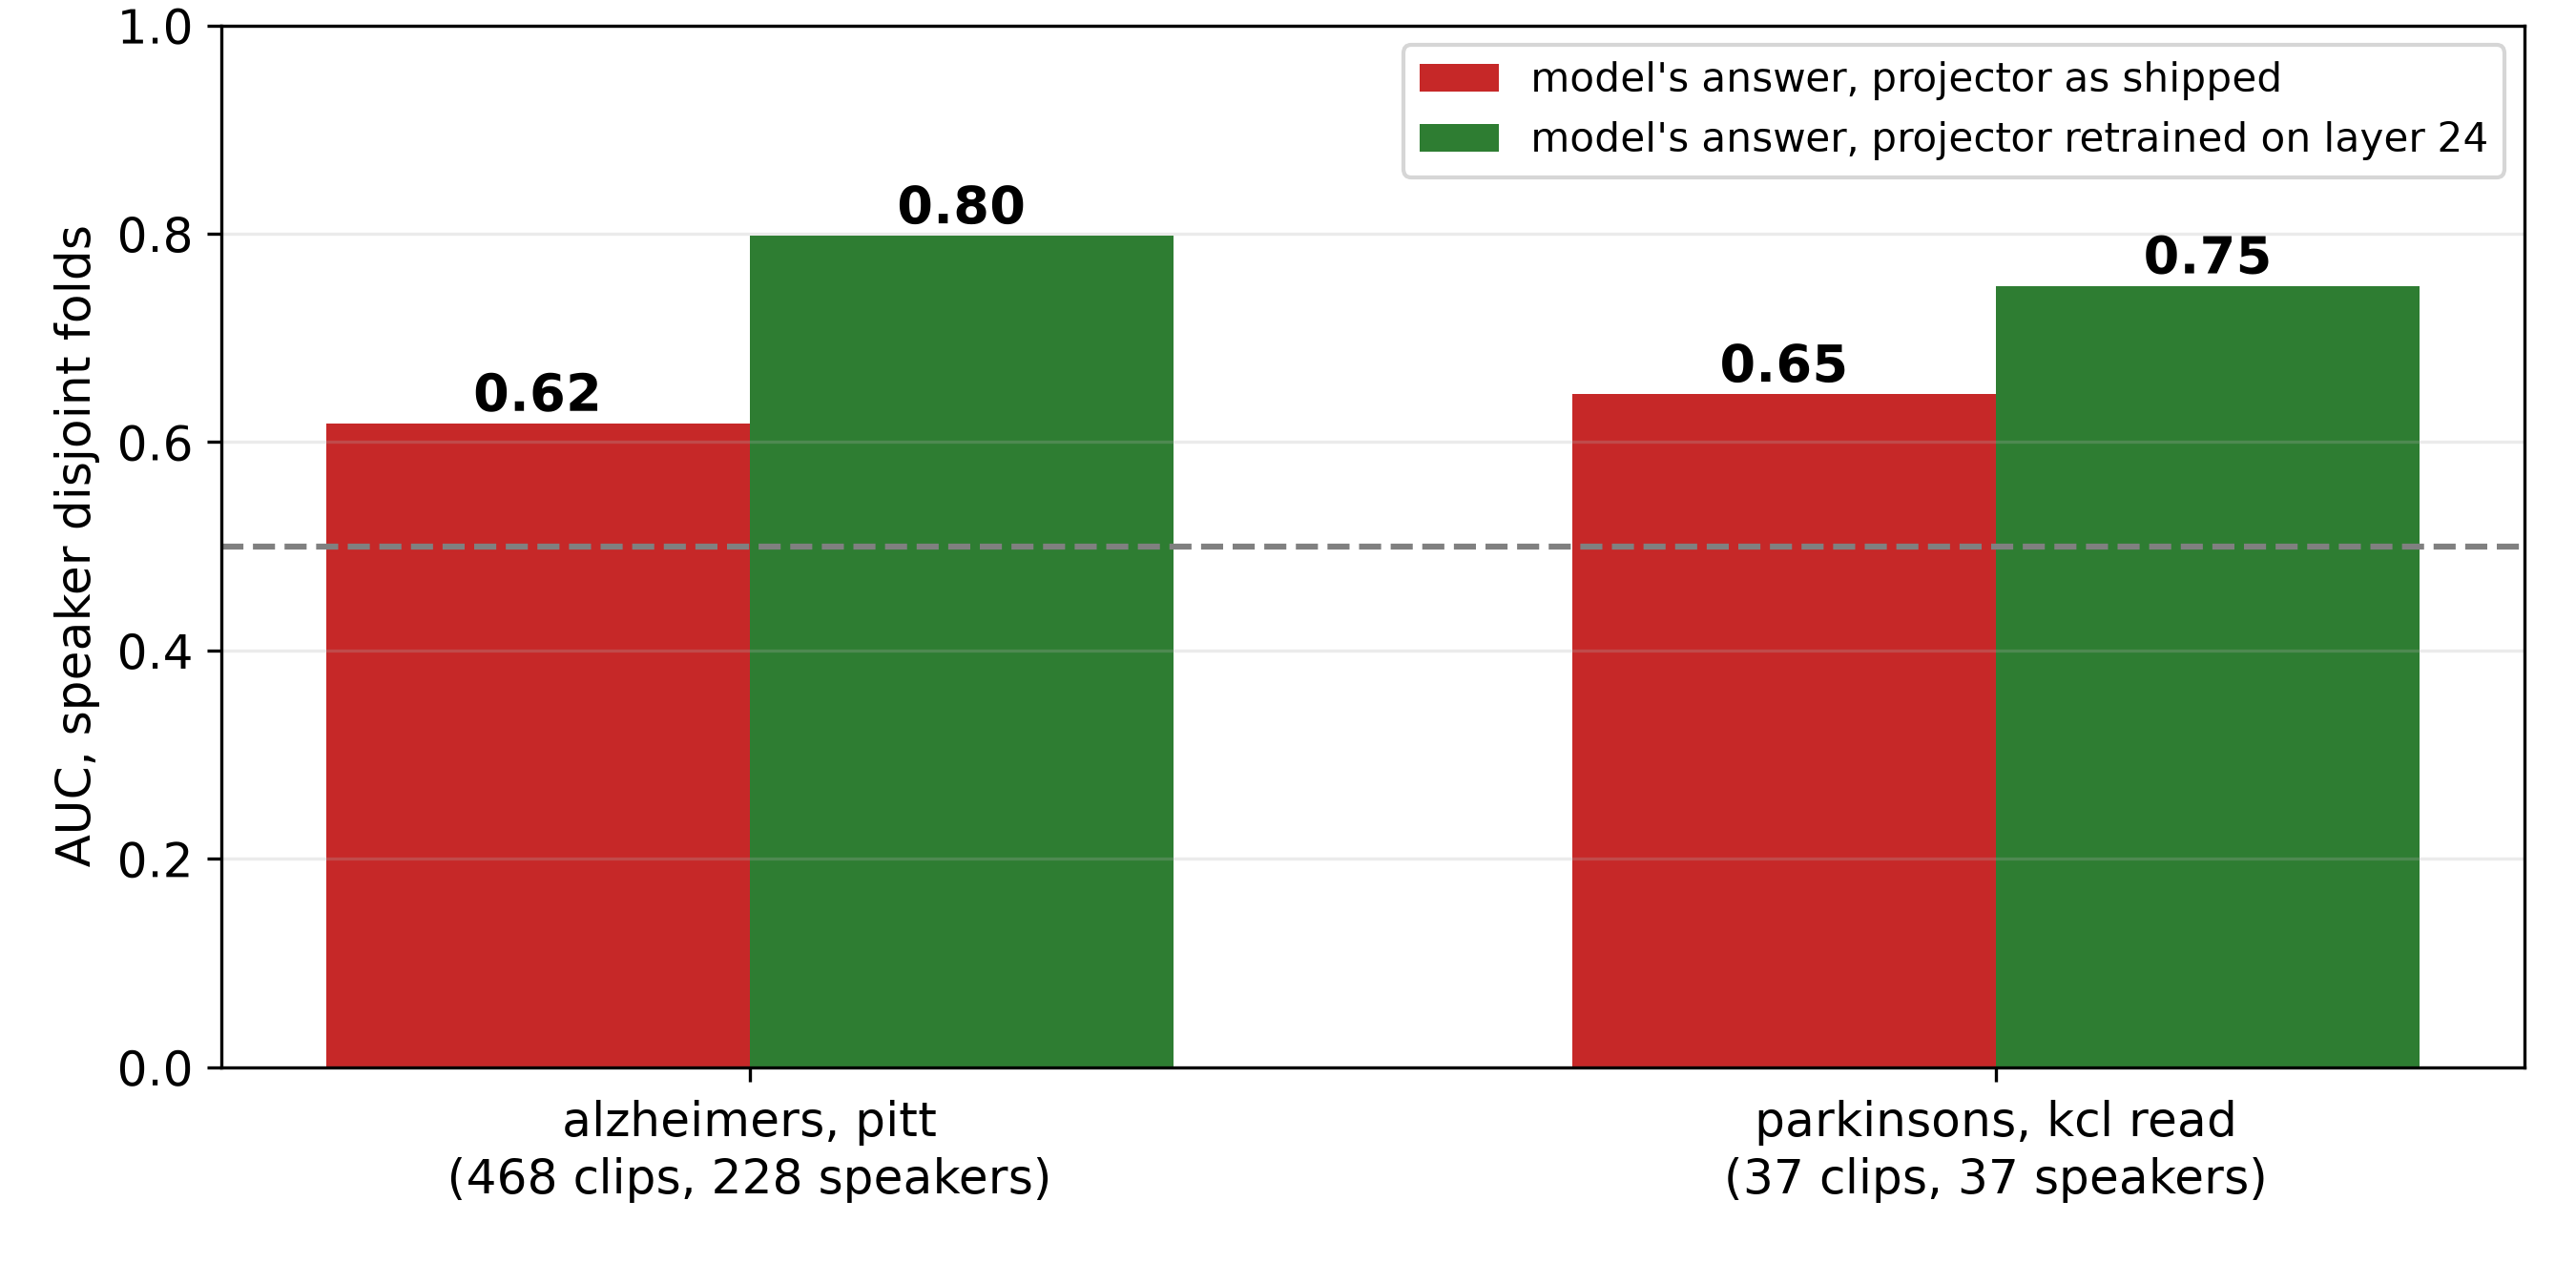
\includegraphics[width=0.64\columnwidth]{plot_projector_two_datasets.png}
\caption{Retraining only the projector, everything else frozen, speaker-disjoint folds. The model's
own answers improve on both diseases. On Alzheimer's the gain is $+0.18$ (95\% interval 0.12 to
0.24); on MDVR-KCL, with 37 speakers, it is $+0.10$ (interval $-0.14$ to $0.35$), a direction rather
than a significant result.}
\label{fig:projector}
\end{figure}

Two interventions train a small component and both close most of the gap. A linear readout on the
frozen hidden states, which is the probe itself, reads 0.78 (interval 0.74 to 0.83) on the Pitt
segments where the answer reads 0.62, a paired gain of $+0.17$ (0.10 to 0.23). Retraining only the
projector, the connector between the audio encoder and the language model, on the diagnosis
answer, with the encoder and the language model frozen and encoder layer 24 as its input, lifts the
model's own answers from 0.62 to 0.80 (0.76 to 0.84), a paired gain of $+0.18$ (0.12 to 0.24), and
from 0.70 to 0.89 on the agreement segments. Retraining the projector on its default input, the final
encoder layer, lifts the answers to 0.76 (0.72 to 0.81; agreement 0.87, conflict 0.48); the layer-24
input adds $+0.035$ ($-0.004$ to $+0.073$) overall and $+0.089$ ($+0.004$ to $+0.177$) on conflict:
the training carries the gain, the earlier layer helps on conflict. On the conflict segments the
readout reaches 0.61 (a
paired gain of $+0.20$, interval 0.04 to 0.34) and the retrained projector 0.57 ($+0.16$, 0.03 to
0.30): both trained fixes move word conflict, and both leave it near 0.6. That the deficit sits in the last step, not earlier, is testable: a probe on the hidden
state at the answer position itself, the vector from which Yes or No is read, reads 0.80 at the final
layer and 0.83 at its best (0.69 on the conflict segments, the highest conflict number in this paper)
while the emitted answer on the same state reads 0.62. The language model integrates the signal; the
projection to the answer tokens discards it. The same projector recipe on MDVR-KCL moves the Parkinson's answers from 0.65, that run's own
baseline, to 0.75 (Figure~\ref{fig:projector}).

\subsection{Other datasets and models}

\begin{table}[t]
\centering\small
\caption{A probe trained on one Parkinson's read-speech dataset and tested cold on another
(qwen2-audio encoder). Diagonal: within-dataset nested values (Section~\ref{sec:gap}). Transfer is
partial and does not follow language: Spanish to Spanish (0.46, 0.66) is worse than Spanish to
English (0.86, 0.74).}
\label{tab:cross}
\begin{tabular}{@{}lccc@{}}
\toprule
trained on, tested on & KCL & Neurovoz & PC-GITA \\
\midrule
KCL       & 0.89 & 0.58 & 0.64 \\
Neurovoz  & 0.74 & 0.96 & 0.66 \\
PC-GITA   & 0.86 & 0.46 & 0.92 \\
\bottomrule
\end{tabular}
\end{table}

On ADReSSo, 237 speakers none of whom appear in Pitt, the probe reaches 0.87 with the layer chosen
inside the training folds (0.89 at the curve's peak) and the model's answer 0.66 (0.59 to 0.73), with
transcript-only input at 0.68. On the ADReSS-2020 benchmark split, with the layer chosen inside the
108 training recordings, the probe reads the 48 test recordings at AUC 0.80 and accuracy 73\%,
against the challenge's own baselines of 62.5\% for acoustic features and 75\% for manual transcripts
\cite{adress2020}. The model's answer reads 0.78 (0.63 to 0.91) on those 48 recordings but 0.62 (0.52
to 0.73) on the 108 training recordings, a swing 48 clips cannot settle, so we pool: over all 156
recordings the probe reads 0.82 with nested layer choice (0.87 at the peak) and the answer 0.68 (0.60
to 0.76). Encoder probes trained on one Parkinson's set and tested cold on another also exist for four
further models, two of them outside the nine (granite speech \cite{granite} and voxtral \cite{voxtral})
plus qwen2.5-omni and diva; with the layer chosen on the training set, Italian excluded, their best
cross-dataset AUCs are 0.81, 0.85, 0.83 and 0.84. Across the Parkinson's sets the probe transfers
across language (Table~\ref{tab:cross}).

\section{Discussion}\label{sec:discussion}

Read together, the results have one shape. The clinical signal is present at every depth of the
model, the answer does not use it, and what the answer uses instead is the words. None of the
training-free fixes raises the conflict answer without destroying the agreement arm; the two fixes
that train one small component lift the Alzheimer's answers to 0.78 and 0.80, and the projector fix
moves the Parkinson's answers in the same direction on a 37-speaker set. The deficit therefore lives
in the readout, not in the representation:
these models are better clinical encoders than clinical reporters, and evaluations that score
their answers only where words and diagnosis agree cannot tell a model that listens from one that
reads.

\noindent\textbf{Limitations.} The layer-wise probing and the fixes are on one model; the nine-model
evidence is the answer-side conflict test. The depression probe and answer coincide at the 30\,s
window, so that condition's claim rests on the conflict construction. MDVR-KCL has 37 speakers, its projector gain is
not significant on its own, and its before number uses the voice wording while the retrained
projector answers the recording wording. ADReSSo transcripts are ASR output (whisper-large-v3), its conflict
group has 19 segments, and the ADReSS-2020 test labels were recovered by matching transcripts to
Pitt (107 of 108 correct and none wrong on the training recordings, whose labels are known), pending
the official labels. The DAIC 30\,s clips were not filtered for
interviewer speech and will be re-cut. On DAIC, scores track PTSD severity
as closely as depression severity (0.60 against 0.59): the models detect distress, not depression
specifically. Pitt and DAIC stay under their own agreements; we release segment identifiers,
scripts and every clip's score.

\clearpage
\begin{table*}[!t]
\centering\small
\caption{Every measurement in one place. Internal review copy, cut before submission.}
\begin{tabular}{@{}p{0.66\textwidth}p{0.30\textwidth}@{}}
\toprule
measurement & AUC \\
\midrule
encoder probe, nested: PC-GITA / Neurovoz / KCL read / Pitt & 0.92 / 0.96 / 0.89 / 0.78 \\
encoder probe, curve peak, Pitt / language-model stages, Pitt & 0.82 / 0.86 \\
model's own answer: PC-GITA / Neurovoz / KCL / DAIC / Pitt & 0.54 / 0.55 / 0.66 / 0.65 / 0.62 \\
answer-position probe, Pitt: final layer / best layer / conflict & 0.80 / 0.83 / 0.69 \\
transcript only, Pitt (clean text) / ADReSSo (whisper-large-v3) & 0.68 / 0.68 \\
DAIC transcript vs own audio answer: $r$ / identical Yes-No & 0.83 / 96\% \\
synthetic voice, Pitt: qwen2-audio / omni / diva / mimo & 0.60 / 0.67 / 0.69 / 0.58 \\
words only, Pitt: qwen2-audio / omni / diva / mimo & 0.72 / 0.72 / 0.71 / 0.57 \\
words check, Pitt: within agreement / on conflict & 0.95 / $\le$0.58 \\
words check, ADReSSo: within agreement / on conflict (n=19) & 0.99 / 0.39 to 0.61 \\
DAIC conflict, nine models: below 0.5 & 6 of 9 \\
Pitt conflict, qwen2-audio: conflict / agreement & 0.41 / 0.70 \\
fixes on conflict: prompts (omni, qwen2-audio) / subtraction / steering / few-shot / plug & 0.34, 0.48 / 0.50 / 0.54 / 0.46 / 0.55 \\
text subtraction at $\alpha = 2.0$: conflict / agreement & 0.67 / 0.18 \\
VoxParadox-recipe checkpoint on conflict: checkpoint / base & 0.37 / 0.35 \\
layer mixer vs one nested layer / prompt-conditioned mixer gain & 0.909 vs 0.916 / +0.0004 \\
trained readout, Pitt: overall / agreement / conflict & 0.78 / 0.86 / 0.61 \\
projector retrained, Pitt: overall / agreement / conflict & 0.80 / 0.89 / 0.57 \\
projector retrained on its default final layer (no plug), Pitt: overall / agreement / conflict & 0.76 / 0.87 / 0.48 \\
layer 24 minus final-layer projector (paired): overall / conflict & +0.035 [$-$0.004, 0.073] / +0.089 [0.004, 0.177] \\
projector retrained, KCL: before / after & 0.65 / 0.75 \\
paired gains, Pitt (95\% intervals): projector / readout & +0.18 [0.12, 0.24] / +0.17 [0.10, 0.23] \\
paired gains on the conflict arm, Pitt: readout / projector & +0.20 [0.04, 0.34] / +0.16 [0.03, 0.30] \\
audio answer minus clean transcript, Pitt (paired) & $-0.06$ [$-0.12$, $+0.01$] \\
ADReSSo: probe nested / probe peak / answer / transcript only & 0.87 / 0.89 / 0.66 / 0.68 \\
ADReSS-2020 official split: probe AUC / accuracy / challenge acoustic, linguistic baselines & 0.80 / 73\% / 62.5\%, 75\% \\
ADReSS-2020 answer: test 48 / train 108 / pooled 156 & 0.78 / 0.62 / 0.68 \\
ADReSS-2020 pooled probe: nested / peak & 0.82 / 0.87 \\
cross dataset, Parkinson's: PC-GITA to KCL / Neurovoz to KCL & 0.86 / 0.74 \\
cross dataset, four further models: granite / voxtral / omni / diva & 0.81 / 0.85 / 0.83 / 0.84 \\
language-model stages on KCL read: min / max & 0.82 / 0.88 \\
classical acoustic floor (eGeMAPS): Pitt / ADReSSo / ADReSS-2020 / KCL & 0.62 / 0.73 / 0.70 / 0.80 \\
recording-only floor: Italian corpus (excluded) / other corpora & 0.995 / 0.45 to 0.80 \\
matched 300\,s window, depression: flamingo 3 / omni / kimi / omni at 30\,s & 0.86 / 0.84 / 0.83 / 0.67 \\
\bottomrule
\end{tabular}
\end{table*}

\bibliographystyle{IEEEtran}
\bibliography{refs}

\end{document}
